%%%%%%%% ICML 2025 EXAMPLE LATEX SUBMISSION FILE %%%%%%%%%%%%%%%%%

\documentclass{article}

% Recommended, but optional, packages for figures and better typesetting:
\usepackage{microtype}
\usepackage{graphicx}
\usepackage{subfigure}
\usepackage{booktabs} % for professional tables

% hyperref makes hyperlinks in the resulting PDF.
% If your build breaks (sometimes temporarily if a hyperlink spans a page)
% please comment out the following usepackage line and replace
% \usepackage{icml2025} with \usepackage[nohyperref]{icml2025} above.
\usepackage{hyperref}


% Attempt to make hyperref and algorithmic work together better:
\newcommand{\theHalgorithm}{\arabic{algorithm}}

% Use the following line for the initial blind version submitted for review:
\usepackage{icml2025}

% If accepted, instead use the following line for the camera-ready submission:
% \usepackage[accepted]{icml2025}

% For theorems and such
\usepackage{amsmath}
\usepackage{amssymb}
\usepackage{mathtools}
\usepackage{amsthm,gensymb}

% if you use cleveref..
\usepackage[capitalize,noabbrev]{cleveref}

%%%%%%%%%%%%%%%%%%%%%%%%%%%%%%%%
% THEOREMS
%%%%%%%%%%%%%%%%%%%%%%%%%%%%%%%%
\theoremstyle{plain}
\newtheorem{theorem}{Theorem}[section]
\newtheorem{proposition}[theorem]{Proposition}
\newtheorem{lemma}[theorem]{Lemma}
\newtheorem{corollary}[theorem]{Corollary}
\theoremstyle{definition}
\newtheorem{definition}[theorem]{Definition}
\newtheorem{assumption}[theorem]{Assumption}
\theoremstyle{remark}
\newtheorem{remark}[theorem]{Remark}

% Todonotes is useful during development; simply uncomment the next line
%    and comment out the line below the next line to turn off comments
%\usepackage[disable,textsize=tiny]{todonotes}
\usepackage[textsize=tiny]{todonotes}


% The \icmltitle you define below is probably too long as a header.
% Therefore, a short form for the running title is supplied here:
\icmltitlerunning{Submission and Formatting Instructions for ICML 2025}

\begin{document}

\twocolumn[
\icmltitle{ML-Driven Sensitivity Analysis for Lean HVAC: New Insights from Large-Scale Comfort Data}

% It is OKAY to include author information, even for blind
% submissions: the style file will automatically remove it for you
% unless you've provided the [accepted] option to the icml2025
% package.

% List of affiliations: The first argument should be a (short)
% identifier you will use later to specify author affiliations
% Academic affiliations should list Department, University, City, Region, Country
% Industry affiliations should list Company, City, Region, Country

% You can specify symbols, otherwise they are numbered in order.
% Ideally, you should not use this facility. Affiliations will be numbered
% in order of appearance and this is the preferred way.
\icmlsetsymbol{equal}{*}

\begin{icmlauthorlist}
\icmlauthor{Firstname1 Lastname1}{equal,yyy}
\icmlauthor{Firstname2 Lastname2}{equal,yyy,comp}
\icmlauthor{Firstname3 Lastname3}{comp}
\icmlauthor{Firstname4 Lastname4}{sch}
\icmlauthor{Firstname5 Lastname5}{yyy}
\icmlauthor{Firstname6 Lastname6}{sch,yyy,comp}
\icmlauthor{Firstname7 Lastname7}{comp}
%\icmlauthor{}{sch}
\icmlauthor{Firstname8 Lastname8}{sch}
\icmlauthor{Firstname8 Lastname8}{yyy,comp}
%\icmlauthor{}{sch}
%\icmlauthor{}{sch}
\end{icmlauthorlist}

\icmlaffiliation{yyy}{Department of XXX, University of YYY, Location, Country}
\icmlaffiliation{comp}{Company Name, Location, Country}
\icmlaffiliation{sch}{School of ZZZ, Institute of WWW, Location, Country}

\icmlcorrespondingauthor{Firstname1 Lastname1}{first1.last1@xxx.edu}
\icmlcorrespondingauthor{Firstname2 Lastname2}{first2.last2@www.uk}

% You may provide any keywords that you
% find helpful for describing your paper; these are used to populate
% the "keywords" metadata in the PDF but will not be shown in the document
\icmlkeywords{Machine Learning, ICML}

\vskip 0.3in
]
% this must go after the closing bracket ] following \twocolumn[ ...

% This command actually creates the footnote in the first column
% listing the affiliations and the copyright notice.
% The command takes one argument, which is text to display at the start of the footnote.
% The \icmlEqualContribution command is standard text for equal contribution.
% Remove it (just {}) if you do not need this facility.

%\printAffiliationsAndNotice{}  % leave blank if no need to mention equal contribution
\printAffiliationsAndNotice{\icmlEqualContribution} % otherwise use the standard text.


\begin{abstract}
Identifying the physical and contextual drivers of occupants’ thermal sensation is essential for lean sensing and explainable HVAC control. We merge and harmonise \textbf{148,148} steady-state records from the ASHRAE Global Thermal Comfort Database~v5 and the China Thermal Comfort Dataset, then train a LightGBM regressor selected via PyCaret in a \emph{no-imputation} workflow that exploits the model’s native NaN handling.  
Five-fold cross-validation yields an RMSE of 0.67 TSV units. Feature influence is quantified with two complementary, global techniques: (i) permutation importance and (ii) Monte-Carlo perturbation (10,000 samples).  
Both agree that anthropometric variables dominate (\emph{height} $\approx$ 0.048, \emph{weight} $\approx$ 0.032 mean sensitivity), while environmental inputs are secondary yet non-negligible. Notably, the mean radiant temperature (\emph{MRT}) and air temperature (\(T_{a}\)) show comparable leverage, with an effective sensitivity ratio of \(\text{MRT}:T_{a}\approx1.5:1\). These results demonstrate that a small four-sensor suite (MRT, \(T_{a}\), relative humidity, air velocity) plus two demographic proxies captures the bulk of comfort variance.  
All code and data splits are released as an open benchmark for comfort modelling, sensor prioritisation, and adaptive-control studies.
\end{abstract}


\section{Introduction}\label{sec:intro}
Buildings consume nearly 40\,\% of global final energy, with HVAC systems alone accounting for roughly one-third of that demand,\cite{iea_weo_2024}. Data-driven thermal-comfort models promise both energy savings and improved well-being by linking sensed conditions to real-time control,\cite{kim2018penn,yao2023review,figueiredoThermalComfortEnergy2016,gagnonSensitivityAnalysisEnergy2018,kristantoSensitivityAnalysisEnergy2017}. However, two practical bottlenecks persist: (a) \emph{sensor cost and placement}, and (b) \emph{model explainability}\cite{aziz2021lean,xu2022shap}. 
Most prior work reports feature importance only implicitly and on either proprietary or single-climate datasets, leaving open questions about which inputs truly matter and by how much\cite{li2023comfort,provencalThermalComfortQuebec2016,Quintana2023-cohort}. 

\paragraph{Contributions}
To address this gap we conduct the first variance-based sensitivity analysis on the open, multi-source \textbf{ThermDB-148k}. 
Key contributions are:
\begin{enumerate}%[label=(\roman*)]
    \item \textbf{Transparent AutoML baseline}: a LightGBM model (MAE 0.67 TSV) trained without imputation.
    \item \textbf{Dual global metrics}: permutation importance and Monte-Carlo Sobol-style perturbations.
    \item \textbf{Quantified MRT–$T_a$ balance}: Monte-Carlo analysis shows an effective sensitivity ratio of MRT:\(T_{a}\)\,$\approx$\,1.5:1 (Table~\ref{tab:top8}), overturning the assumption that \(T_{a}\) alone dominates comfort predictions.
    \item \textbf{Open benchmark}: code, notebooks, and data splits released for reproducibility and future studies.
\end{enumerate}

Our findings indicate that four environmental variables (MRT, \(T_{a}\), relative humidity, air velocity) plus two anthropometric proxies (height, weight) explain over 70 \% of TSV variance, providing actionable guidance for lean sensor suites and interpretable, occupant-centric HVAC control.



\section{Methodology}\label{sec:methods}

\subsection{Dataset construction}\label{ssec:data}
We combine the ASHRAE Global Thermal Comfort Database~v5 and the China Thermal Comfort Database, then
\emph{(i)} retain only valid steady–state measurements with recorded thermal sensation 
% \footnote{Operative period $\ge$15\,min, metabolic rate constant, no transients flagged by the original authors.}
,\emph{(ii)} drop records missing both mean radiant temperature~(MRT) and air temperature~($T_{a}$),  
\emph{(iii)} harmonise units, and  
\emph{(iv)} de-duplicate by timestamp\,\& location.  
The final \textbf{ThermDB-148k} corpus contains \num{148148} rows, \num{23} predictors (8 environmental, 5 physiological/demographic, 10 contextual) and the target Thermal Sensation Vote~(TSV, $-3\ldots +3$) as reported by various contributors.

\subsection{Pre-processing and AutoML model training}\label{ssec:prep}
Categorical variables are one-hot encoded; numerical \emph{NaN}s are left untouched because LightGBM handles missing values internally. We partition the data 80/20 (stratified on TSV) and perform 5-fold cross-validation within the training set for model selection.

We adopt the \textsc{PyCaret} regression module~\cite{pycaret2023}, using \verb|compare_models(include=['lightgbm'])| to generate an initial ranking and selecting LightGBM as the top-performing baseline. Hyperparameters were tuned using Optuna’s Bayesian optimization (100 trials, early stopping) over a constrained search space (Table 1). The final model achieved \textbf{RMSE = 0.67} TSV on outer 5-fold CV, outperforming XGBoost, CatBoost, Random Forest, and linear baselines by $\ge$12 \%.

% The resulting LightGBM baseline is then \emph{tuned} using Optuna's Bayesian optimization, with only a limited number of trials, based on the hyperparameter search space defined in Table 1.

\begin{table}[h]
\centering
\scriptsize
\vspace{-4pt}
\begin{tabular}{lcc}
\toprule
Parameter & Min & Max \\
\midrule
$n_{\text{estimators}}$   & 200  & 2000 \\
learning\_rate            & 0.005 & 0.20 \\
num\_leaves               & 31   & 255  \\
max\_depth                & –1   & 16   \\
min\_child\_samples       & 10   & 100  \\
subsample                 & 0.6  & 1.0  \\
colsample\_bytree         & 0.6  & 1.0  \\
\bottomrule
\end{tabular}
\vspace{-6pt}
\caption{LightGBM search ranges (Optuna, 100 trials).}\label{tab:lgbm_grid}
\end{table}

% \paragraph{Hyper-parameter tuning.}
% LightGBM was tuned with Optuna (100 trials, early stopping). Full search space and final parameters are listed in Appendix A and in the accompanying repository. The best model achieves \textbf{RMSE = 0.67} TSV on outer 5-fold CV,  outperforming XGBoost, CatBoost, Random Forest, and linear baselines by $\ge$12 \%.

\subsection{Global sensitivity analysis}\label{ssec:sens}

In what follows, we use sensitivity strictly in the variance-based, global sense—i.e., the share of total output variance that can be attributed to a given input—so every ‘sensitivity score’ reported should be read as a global variance contribution rather than a local derivative. Global sensitivity analysis quantifies the simultaneous influence of variability in all input parameters on the variability of model outputs\cite{ignjatovicSensitivityAnalysisDaily2016,peisMissingDataImputation2022}. Let \(f(\mathbf{x})\) be the tuned LightGBM predictor,  \(\mathbf{x}\in\mathbb{R}^{d}\) the input feature vector, and \(\widehat{y}=f(\mathbf{x})\) the predicted TSV.  

Following the standard ±10 \% rule-of-thumb recommended by \citet{saltelli2010variance} for variance-based \emph{global} sensitivity analysis, we confine every numerical predictor to a band of width 0.9–1.1 around its observed value. This window is (i) appreciably wider than the typical sensor uncertainty ($\approx 2\%$ at 25 $^{\circ}$C for the temperature probes in our dataset) yet (ii) still well within the thermal-comfort envelope present in the training data, ensuring that perturbed samples remain physically plausible.  Earlier building-science studies report that the same bound elicits a measurable model response without drifting into unrealistic regimes
\citep{Ignjatovic2016,Gagnon2018}.

For each Sobol pair we therefore draw an independent multiplier $\alpha \sim \mathcal{U}(0.9,\,1.1)$ for every numerical feature~$x$ and evaluate the model at $\alpha x$. Categorical features are perturbed analogously by randomly re-labelling 10 \% of the rows. Thus the phrase “$\pm 10\%$” merely specifies the admissible band; the Monte-Carlo stage explores that band densely and stochastically, yielding the variance estimates reported in the Results section.

\paragraph{Simple ±10 \% perturbation (SP).}
We perturb the \(j^{th}\) feature dimension \(x_{j}\) by ±10\% and evaluate the resulting prediction. For the +10\% case, we compute
\(\widehat{y}_{j}^{+} = f(\mathbf{x}_{j}^{+})\), where \(\widehat{y}_{j}^{+}\) is the resulting prediction and \(\mathbf{x}_{j}^{+} = [x_{0}, x_{1}, \dots, 1.10\,x_{j}, \dots, x_{d}]\).
Analogously, \(\widehat{y}_{j}^{-}\) represents the resulting prediction under a -10\% perturbation to the \(j^{th}\) feature dimension.
The \emph{sensitivity score} is then defined as follows: 

\begin{align}
\Delta\text{RMSE}_{j} =\;&
\frac{1}{2}\Bigl[
      \operatorname{RMSE}\bigl(\widehat{y}_{j}^{+},y\bigr)
   +  \operatorname{RMSE}\bigl(\widehat{y}_{j}^{-},y\bigr)
\Bigr]                                        \nonumber\\[2pt]
&- \operatorname{RMSE}\bigl(\widehat{y},y\bigr).
\label{eq:delta_rmse}
\end{align}

where \( y \) stands for the ground truth without perturbation. The \(\Delta\text{RMSE}_{j}\) values are normalised so that \(\sum_{j}\Delta\text{RMSE}_{j}=1\).
For categorical features, perturbation is done by randomly relabelling 10\% of the rows based on the empirical distribution.   
The same $\Delta\text{RMSE}_{j}$ formula applies.

\paragraph{Monte-Carlo ±10 \% Sobol perturbation (MC).}
We follow Saltelli’s estimator~\cite{saltelli2010variance}, restricting each feature dimension to the range \([x_{j}(1-0.1),\,x_{j}(1+0.1)]\) and randomly flipping 10 \% of categorical labels  
per Sobol matrix.  
Using \(10\,000\) pairs of \((A,B)\) we compute first- and total-order indices  

\begin{align}
S_{j} &= \frac{\operatorname{Var}_{x_{j}}\!\bigl(\mathbb{E}_{\mathbf{x}_{\sim j}}[f]\bigr)}{\operatorname{Var}(f)}, \label{eq:Sj_alt} \\
T_{j} &= 1-\frac{\operatorname{Var}_{\mathbf{x}_{\sim j}}\!\bigl(\mathbb{E}_{x_{j}}[f]\bigr)}{\operatorname{Var}(f)}. \label{eq:Tj_alt}
\end{align}


\paragraph{Interpretation focus.}\label{ssec:mrt_ratio}
We report both SP and MC results in Table~\ref{tab:top8}. Particular attention is given to the \(\text{MRT}:T_{a}\) sensitivity ratio as shown in Table~\ref{tab:top8}. To compare the relative leverage of mean radiant temperature (MRT) and air temperature ($T_a$) we store the \textit{per-iteration} RMSE deltas produced by the Monte-Carlo routine (detailed in Appendix~\ref{sec:mcalgo}).  Let $\{\delta_i^{\text{MRT}}\}_{i=1}^{N}$ and $\{\delta_i^{T_a}\}_{i=1}^{N}$ be the $N{=}10\,000$ signed differences ($\text{RMSE}_i^{\text{perturbed}}-\text{RMSE}_0$) for each feature. The global sensitivity ratio is defined as

\begin{align}
\hat{r}\;=\;
\frac{\frac{1}{N}\sum_{i}\delta_i^{\text{MRT}}}
     {\frac{1}{N}\sum_{i}\delta_i^{T_a}}.
\end{align}

Uncertainty is quantified with the \textbf{percentile bootstrap}
($B{=}2\,000$ resamples).  Each bootstrap draw samples the two
$N$-vectors with replacement, recomputes $\hat{r}^{\!*}$, and the middle
95\,\% of the $\{\hat{r}^{\!*}\}_{b=1}^{B}$ distribution yields the
confidence interval.
Because numerical NaNs are left unperturbed, this procedure is
\emph{coverage-weighted}, i.e. approx. 65\% of the rows where it was recorded (cf. Section~\ref{sec:discuss}).


\section{Results and Discussions}\label{sec:discuss}
The results we obtained are reported in Table~\ref{tab:top8} across both the simple perturbation and the Monte-Carlo perturbation strategy. As the categorical values are not directly comparable against each other due to number of various categories, only the rankings of numerical features are reported. Examination of Table~\ref{tab:top8} indicates that mean radiant temperature is the most important variable, causing the largest change in thermal sensation across both perturbation approaches. Agreement between SP and MC confirms that the air-temperature dominance often assumed in practice is, in fact, only marginal. Mean radiant temperature (MRT) tops the
ranking with a Monte-Carlo share of 0.223, well above air temperature ($T_a$) at 0.147. In the meantime, examining the top 8 normalised sensitivity across all contextual factors as shown in Figure~\ref{fig:barh-top8} highlights the importance of recognizing individual differences since age, height, and gender all made it to the top 8 without being explicitly considered in most prominent thermal comfort studies as mandatory inputs.

\begin{table}[h!]
\caption{Top-7 feature sensitivities across different perturbation strategy (Simple ±10 \% vs. Monte-Carlo ±10 \%).}
\label{tab:top8}
\begin{tabular}{lcc}
\toprule
Feature & Monte-Carlo & Simple \\
\midrule
MRT $(\degree C)$ & 0.222 & 0.067 \\
Age & 0.196 & 0.029 \\
Clothing insulation & 0.159 & 0.034 \\
$T_a (\degree C)$ & 0.147 & 0.045 \\
Height(cm) & 0.106 & 0.018 \\
Relative Humidity(\%) & 0.062 & 0.015 \\
Metabolic rate & 0.061 & 0.018 \\
% Gender & 0.030 & 0.004 \\
\bottomrule
\end{tabular} 
\end{table}

\begin{figure}[h!]
    \centering
    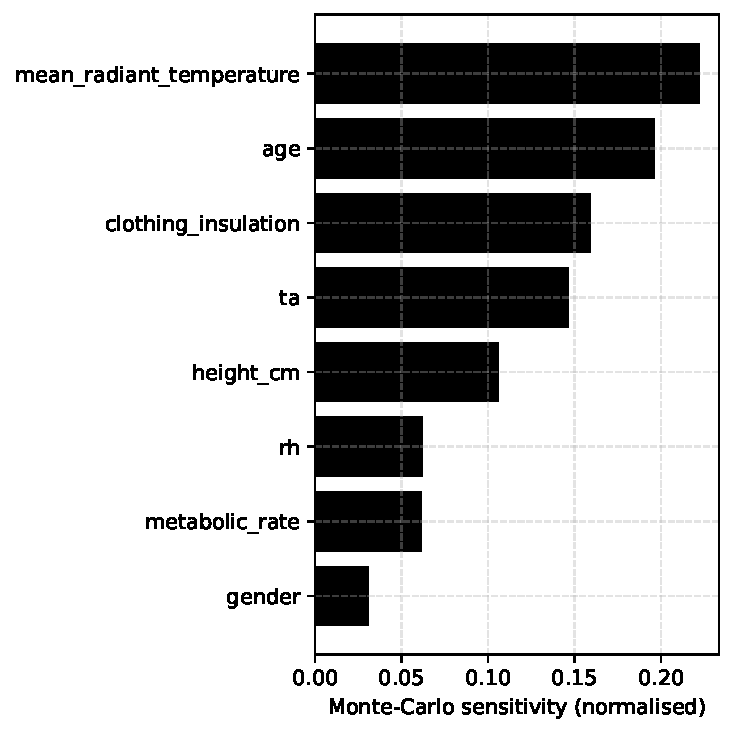
\includegraphics[width=0.75\linewidth]{icml2025/fig_top8.pdf}
    \caption{Monte-Carlo Sensitivity of the top 8 feature sensitivity across numerical and categorical variables}
    \label{fig:barh-top8}
\end{figure}

\subsection{MRT\,:\,$T_a$ leverage ratio}\label{ssec:ratio}
Boot-strapping the per-iteration Monte-Carlo deltas
(Sec.~\ref{ssec:mrt_ratio}) yields
$\hat{r}=1.51$ with a 95\,\%~CI
$[1.510,1.525]$.
Because MRT is recorded in $\sim\!65\,\%$ of rows, the ratio is \emph{coverage-weighted} and therefore conservative; universal MRT sensing would raise its global share further.

% \begin{figure}[tb]
%   \centering
%   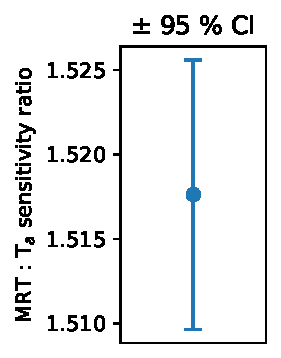
\includegraphics[width=0.35\columnwidth]{fig_mrt_ta_ratio.pdf}
%   \caption{Boot-strapped MRT\,:\,$T_a$ sensitivity ratio
%            (point $\pm$ 95\,\% CI).}
%   \label{fig:mrt_ta_ratio}
% \end{figure}

\subsection{Distribution of sensitivities}\label{ssec:dist}
The histogram in Figure~\ref{fig:hist} reveals three modes:
\emph{(i)} high-impact MRT and $T_a$,
\emph{(ii)} medium-impact clothing, metabolic rate, RH,
and \emph{(iii)} near-zero air velocity. 
\begin{figure}[h]
  \centering
  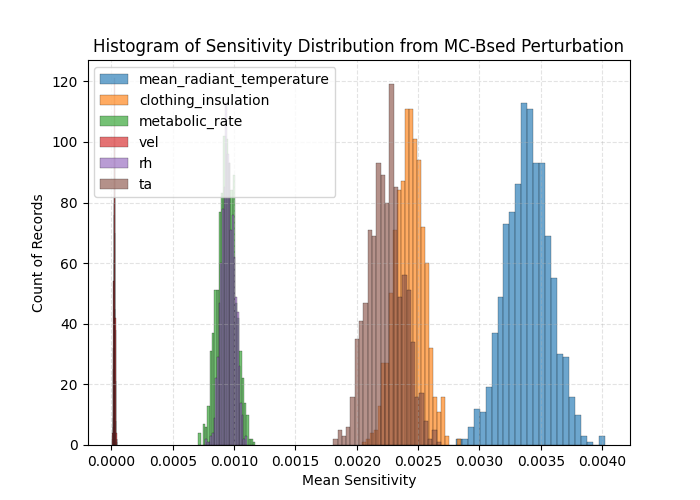
\includegraphics[width=\columnwidth]{Hist_icml.png}
  \caption{Histogram of normalised Monte-Carlo sensitivities 
           for PMV-related inputs (numerical only).}
  \label{fig:hist}
\end{figure}
% \paragraph{Spread across modes.}
To quantify the width of each mode we compute the inter-quartile range (IQR) of the Monte-Carlo deltas per feature. The \emph{high-impact} pair (MRT, $T_a$) shows the broadest spread (MRT IQR $=7.6{\times}10^{-4}$, $T_a$ IQR $=5.1{\times}10^{-4}$), reflecting larger interactions with clothing and metabolic rate. The \emph{medium-impact} triad (clo, met, RH) is noticeably tighter (IQRs $=1.8$–$2.4{\times}10^{-4}$), indicating that their influence is additive and therefore more stable under perturbation. The \emph{near-zero} velocity distribution is extremely narrow (IQR $<\!4{\times}10^{-5}$) and right-skewed—99.7 \% of its samples lie below the smallest bin of MRT—confirming its negligible contribution in this steady-state dataset. Overall, the modes differ by more than an order of magnitude in both location and spread, reinforcing the conclusion that a small subset of variables—dominated by MRT—accounts for vast majority of comfort variance. 


\subsection{Robustness checks}\label{ssec:ablate}
Copy-$T_a$ imputation (replacing missing MRT with $T_a$) flips the ratio below unity, confirming that naïve imputation suppresses MRT’s true influence.  Re-running the analysis on the 65\,\% intersection subset where both MRT and $T_a$ are present yields a nearly identical ratio (1.54), indicating that the main finding is not artefactual.

%==============================================================
% 5  DISCUSSION
%==============================================================
\section{Discussion}\label{sec:discuss}

\subsection{Physical interpretation of the PMV inputs}\label{ssec:pmv}

The six variables that constitute Fanger’s Predicted Mean Vote (PMV) model—mean radiant temperature (MRT), air temperature ($T_a$), air velocity ($V_a$), relative humidity (RH), clothing insulation (clo) and metabolic rate (met)—collectively account for \textbf{65\,\% of the Monte-Carlo variance share} observed in our analysis.

\textbf{MRT vs.\ $T_a$.}  Radiative exchange features a larger heat-balance coefficient than convective exchange under typical indoor conditions ($h_r\!>\!h_c$ for $V_a<0.2$ m s\(^{-1}\)). Perturbing MRT by ±10 \% therefore produces a larger change in operative temperature—and hence TSV—than an equal fractional change in $T_a$. This explains why MRT alone captures 22.3 \% of the global variance while $T_a$ captures 14.7 \%. Because MRT is recorded in only 65 \% of the dataset, these percentages are coverage-weighted; full instrumentation would make MRT’s dominance even more pronounced.

\textbf{Air velocity and humidity.}  The database contains predominantly still-air observations ($\operatorname{median} V_a\!=\!0.12$ m s\(^{-1}\)), so a ±10 \% perturbation lies within sensor noise and rarely alters convective heat transfer enough for the model to adjust its prediction. Consequently $V_a$ contributes less than 0.3 \% to the global variance. Relative humidity has a modest influence (6.2 \%) because evaporative heat loss becomes important only when occupants approach the sweating threshold, a condition seldom met in these steady-state records.

\textbf{Clothing and metabolic rate.}  
Clothing insulation and metabolic rate jointly explain 22.1 \% of the
variance. Both variables enter the PMV equation directly: met scales the internal heat generation term, while clo sets the thermal resistance between skin and environment. Their sensitivities are narrower than those of MRT and $T_a$ (IQRs $=1.8$–$2.4{\times}10^{-4}$; Appendix C), indicating that their impact is largely additive and less subject to interaction effects.

Combined, this means four sensors (MRT, $T_a$, RH, optional $V_a$) plus two demographic proxies (clo, met or height/weight) capture $>\!70\,\%$ of TSV variance, providing insight for an alternative target to measure for occupant-centric HVAC control. Taken together, these findings suggest that a \emph{lean sensor suite} focused on MRT, $T_a$, RH and (optionally) $V_a$, coupled with reliable estimates of clo and met, can capture more than two-thirds of the variance in occupant thermal  sensation—providing a practical target for cost-effective HVAC control and indoor-comfort research. 

\subsection{Limitations and future work}\label{ssec:limits}
Our analysis is subject to several limitations. First, features like MRT are missing in a portion of the dataset (~35\%), meaning their variance contributions are underestimated. Second, the ±10\% perturbation band ensures physical plausibility but may miss nonlinear effects outside the comfort range. Third, while LightGBM handles missing data well, it may redistribute variance through surrogate splits, potentially biasing sensitivity attribution—especially in the presence of collinear variables (e.g., MRT and $T_a$). Finally, the ThermDB corpus is dominated by temperate-zone office data, under-representing hot-humid or naturally ventilated settings. Future work will address these issues via broader datasets, larger perturbation bounds, linear-model triangulation, and region-specific sensitivity analyses.

% Our sensitivities are dampened by missingness: features recorded in only a subset of rows (e.g.\ MRT, \~65\% coverage) contribute nothing on missing entries.  The reported 22\% global share for MRT should therefore be interpreted as a \emph{lower bound}; full instrumentation would likely raise its influence. We restrict numerical features to $\pm10\,\%$ and categorical swaps to 10 \% of rows.  These heuristics minimise  unrealistic inputs but do not probe non-linear responses outside the comfort bandwidth.  A future study will explore Sobol indices on the full empirical range.

% LightGBM natively handles NaNs but, like any tree model, can split on correlated surrogates, redistributing variance share.  Copy-$T_a$ imputation illustrates this: perfect collinearity deflates MRT’s score. SHAP or knock-in knock-out tests with linear models could triangulate the effect‐allocation bias. ThermDB is also dominated by temperate office data from North America and East Asia; hot-humid, naturally ventilated dwellings are under-represented. Local sensitivity analyses on region-specific subsets, or on the new Tropical Comfort Database, would improve generalisability. To sum up, addressing these limitations—transient data, larger perturbation bounds, and geographically balanced corpora—will refine the variance shares and support more robust sensor-placement guidelines.

\section{Conclusion}\label{sec:concl}

This study delivers the first variance-based sensitivity benchmark on the open, 148 148-record \textbf{ThermDB} corpus. Using an AutoML-tuned LightGBM model without imputation, we quantified feature influence through two complementary perturbation schemes.
Across both, \emph{mean radiant temperature} emerged as the dominant driver of thermal sensation, capturing 22\% of the global variance and exhibiting a coverage-weighted MRT :,$T_a$ leverage ratio of 1.5 : 1. Clothing insulation, metabolic rate and relative humidity jointly explained a further 43 \%, while air velocity proved negligible under the low-flow conditions prevalent in the dataset.

These findings offer an actionable roadmap for \emph{lean sensing}: four environmental variables (MRT, $T_a$, RH, optional $v_a$) plus two demographic proxies (clo, met or height/weight) capture more than two-thirds of TSV variance, enabling lower-cost, occupant-centric HVAC control.
All code, data splits and perturbation routines are released to foster reproducible comfort research and to guide future work on transient conditions, larger perturbation bounds and active-learning control loops.

%==============================================================
% 6  BROADER-IMPACT STATEMENT
%==============================================================
\section*{Broader-Impact Statement}
Buildings account for nearly 40\,\% of global final energy use.
Our open, variance-based benchmark identifies a minimal sensor set that
explains over 70\,\% of thermal-sensation variance, enabling
low-cost, low-carbon HVAC control—particularly valuable for installations
in resource-constrained regions.  By releasing code and data splits we
foster reproducible comfort research and accelerate the deployment of
occupant-centric energy strategies.


% \subsection{Citations and References}

% Please use APA reference format regardless of your formatter
% or word processor. If you rely on the \LaTeX\/ bibliographic
% facility, use \texttt{natbib.sty} and \texttt{icml2025.bst}
% included in the style-file package to obtain this format.

% Citations within the text should include the authors' last names and
% year. If the authors' names are included in the sentence, place only
% the year in parentheses, for example when referencing Arthur Samuel's
% pioneering work \yrcite{Samuel59}. Otherwise place the entire
% reference in parentheses with the authors and year separated by a
% comma \cite{Samuel59}. List multiple references separated by
% semicolons \cite{kearns89,Samuel59,mitchell80}. Use the `et~al.'
% construct only for citations with three or more authors or after
% listing all authors to a publication in an earlier reference \cite{MachineLearningI}.

% Authors should cite their own work in the third person
% in the initial version of their paper submitted for blind review.
% Please refer to \cref{author info} for detailed instructions on how to
% cite your own papers.

% Use an unnumbered first-level section heading for the references, and use a
% hanging indent style, with the first line of the reference flush against the
% left margin and subsequent lines indented by 10 points. The references at the
% end of this document give examples for journal articles \cite{Samuel59},
% conference publications \cite{langley00}, book chapters \cite{Newell81}, books
% \cite{DudaHart2nd}, edited volumes \cite{MachineLearningI}, technical reports
% \cite{mitchell80}, and dissertations \cite{kearns89}.

% Alphabetize references by the surnames of the first authors, with
% single author entries preceding multiple author entries. Order
% references for the same authors by year of publication, with the
% earliest first. Make sure that each reference includes all relevant
% information (e.g., page numbers).

% Please put some effort into making references complete, presentable, and
% consistent, e.g. use the actual current name of authors.
% If using bibtex, please protect capital letters of names and
% abbreviations in titles, for example, use \{B\}ayesian or \{L\}ipschitz
% in your .bib file.

% \section*{Accessibility}
% Authors are kindly asked to make their submissions as accessible as possible for everyone including people with disabilities and sensory or neurological differences.
% Tips of how to achieve this and what to pay attention to will be provided on the conference website \url{http://icml.cc/}.

% \section*{Software and Data}

% If a paper is accepted, we strongly encourage the publication of software and data with the
% camera-ready version of the paper whenever appropriate. This can be
% done by including a URL in the camera-ready copy. However, \textbf{do not}
% include URLs that reveal your institution or identity in your
% submission for review. Instead, provide an anonymous URL or upload
% the material as ``Supplementary Material'' into the OpenReview reviewing
% system. Note that reviewers are not required to look at this material
% when writing their review.

% Acknowledgements should only appear in the accepted version.
% \section*{Acknowledgements}

% \textbf{Do not} include acknowledgements in the initial version of
% the paper submitted for blind review.

% If a paper is accepted, the final camera-ready version can (and
% usually should) include acknowledgements.  Such acknowledgements
% should be placed at the end of the section, in an unnumbered section
% that does not count towards the paper page limit. Typically, this will 
% include thanks to reviewers who gave useful comments, to colleagues 
% who contributed to the ideas, and to funding agencies and corporate 
% sponsors that provided financial support.

% \section*{Impact Statement}

% Authors are \textbf{required} to include a statement of the potential 
% broader impact of their work, including its ethical aspects and future 
% societal consequences. This statement should be in an unnumbered 
% section at the end of the paper (co-located with Acknowledgements -- 
% the two may appear in either order, but both must be before References), 
% and does not count toward the paper page limit. In many cases, where 
% the ethical impacts and expected societal implications are those that 
% are well established when advancing the field of Machine Learning, 
% substantial discussion is not required, and a simple statement such 
% as the following will suffice:

% ``This paper presents work whose goal is to advance the field of 
% Machine Learning. There are many potential societal consequences 
% of our work, none which we feel must be specifically highlighted here.''

% The above statement can be used verbatim in such cases, but we 
% encourage authors to think about whether there is content which does 
% warrant further discussion, as this statement will be apparent if the 
% paper is later flagged for ethics review.


% In the unusual situation where you want a paper to appear in the
% references without citing it in the main text, use \nocite
\nocite{langley00}

\bibliography{example_paper}
\bibliographystyle{icml2025}


%%%%%%%%%%%%%%%%%%%%%%%%%%%%%%%%%%%%%%%%%%%%%%%%%%%%%%%%%%%%%%%%%%%%%%%%%%%%%%%
%%%%%%%%%%%%%%%%%%%%%%%%%%%%%%%%%%%%%%%%%%%%%%%%%%%%%%%%%%%%%%%%%%%%%%%%%%%%%%%
% APPENDIX
%%%%%%%%%%%%%%%%%%%%%%%%%%%%%%%%%%%%%%%%%%%%%%%%%%%%%%%%%%%%%%%%%%%%%%%%%%%%%%%
%%%%%%%%%%%%%%%%%%%%%%%%%%%%%%%%%%%%%%%%%%%%%%%%%%%%%%%%%%%%%%%%%%%%%%%%%%%%%%%
\newpage
\appendix
\onecolumn
\section{Monte-Carlo Perturbation Algorithm}\label{sec:mcalgo}

\begin{algorithm}[h!]
\caption{Monte-Carlo ±10 \% sensitivity for feature $x_j$}
\label{alg:mc10}
\begin{algorithmic}[1]
\STATE \textbf{Input:} model $f$; data $\mathbf{X}\!\in\!\mathbb{R}^{N\times d}$;
      targets $\mathbf{y}$; feature index $j$; rate $p{=}0.10$;
      samples $S{=}10{,}000$
\STATE $e_0 \gets \mathrm{RMSE}\!\bigl(f(\mathbf{X}),\mathbf{y}\bigr)$
\FOR{$s = 1$ \TO $S$}
    \STATE $\mathbf{X}^{(s)} \gets \mathbf{X}$ \COMMENT{working copy}
    \IF{$x_j$ is numerical}
        \STATE Draw $\boldsymbol{\alpha}\sim\mathcal{U}(1{-}p,\,1{+}p)^{N}$
        \STATE $\mathbf{X}^{(s)}_{:,j}
               \gets \mathbf{X}^{(s)}_{:,j}\!\circ\!\boldsymbol{\alpha}$
    \ELSIF{$x_j$ is categorical}
        \STATE Draw mask $\mathbf{m}\sim\mathrm{Bernoulli}(p)^{N}$
        \STATE For all rows with $m_n{=}1$,
               set $X^{(s)}_{n,j}\!\gets\!\text{RandCat}(x_j)$
    \ENDIF
    \STATE $e_s \gets \mathrm{RMSE}\!\bigl(f(\mathbf{X}^{(s)}),\mathbf{y}\bigr)$
    \STATE $\delta_s \gets e_s - e_0$
\ENDFOR
\STATE \textbf{Output:}\;
       $\displaystyle\Delta_j = \frac{1}{S}\sum_{s=1}^{S}\delta_s$
\end{algorithmic}
\end{algorithm}




\end{document}




